%% LyX 2.5.1 created this file.  For more info, see https://www.lyx.org/.
%% Do not edit unless you really know what you are doing.
\documentclass[english]{article}
\usepackage{courier}
\usepackage[T1]{fontenc}
\usepackage[latin9]{inputenc}
\usepackage[table]{xcolor}
\usepackage{colortbl}
\usepackage{babel}
\usepackage{cprotect}
\usepackage{enumitem}
\usepackage{amsmath}
\usepackage{amsthm}
\usepackage{graphicx}
\usepackage{geometry}
\geometry{verbose,tmargin=1in,bmargin=1in,lmargin=1in,rmargin=1in}
\usepackage[pdfusetitle,
 bookmarks=true,bookmarksnumbered=false,bookmarksopen=false,
 breaklinks=false,pdfborder={0 0 1},backref=false,colorlinks=false]
 {hyperref}

\makeatletter

%%%%%%%%%%%%%%%%%%%%%%%%%%%%%% LyX specific LaTeX commands.
%% Because html converters don't know tabularnewline
\providecommand{\tabularnewline}{\\}

%%%%%%%%%%%%%%%%%%%%%%%%%%%%%% Textclass specific LaTeX commands.
\newlength{\lyxlabelwidth}      % auxiliary length 

\ifdefined\showcaptionsetup
 % Caption package is used. Advise subfig not to load it again.
 \PassOptionsToPackage{caption=false}{subfig}
\fi
\usepackage{subfig}
\makeatother

\theoremstyle{plain}
\newtheorem{thm}{\protect\theoremname}
\newtheorem{question}[thm]{\protect\questionname}
\theoremstyle{definition}
\newtheorem*{sol*}{\protect\solutionname}
\usepackage{listings}
\providecommand{\questionname}{Question}
\providecommand{\solutionname}{Solution}
\providecommand{\theoremname}{Theorem}
\renewcommand{\lstlistingname}{Listing}

\begin{document}
\title{Assignment \#1}
\date{Due: 13th of February 2026\\
}
\author{Jonathan Horton (\#7710257)}
\maketitle

\section{Architecture and Computer/GPU Details }

The architecture used for both JAX and Pytorch is a simple feed forward
network with 4 layers of sizes 784, 256, 128, and 10. Each neuron
uses a ReLU activation function. The cross entropy loss was used along
with an accuracy measurement to determine model performance. An 80-20
training-validations split was used.

The code was run on a computer with 32 GB of RAM, a AMD Ryzen 9 3900X
12-Core 3.80GHz Processor, and on a NVIDIA GeForce RTX 2080 (8GB)
GPU.

\section{Performance Comparison and Conceptual Discussion}
\begin{question}
How does JAX\textquoteright s functional programming paradigm differ
from PyTorch/TensorFlow?
\end{question}

\begin{sol*}
JAX uses a functional programming approach, whereas Pytorch/Tensorflow
use an object oriented programming approach. JAX does not have a built
in neural network library. It's parameters are managed manually or
using external libraries like the one mentioned in the assignment
instructions, Flax. Regardless, both libraries allow for custom neural
network architectures. Jax is primarily suited for research, and Pytorch
is an older library that is used in production workflows. Jax has
been shown to outperform Pytorch in a number of benchmarks and areas.
Libraries like TorchServe make it Torch much better suited to integrated
with systems for MLOps. {[}1{]}
\end{sol*}
\begin{question}
Discuss the role of \lstinline[language=Python,basicstyle={\ttfamily}]!jit!
and \lstinline[language=Python,basicstyle={\ttfamily}]!grad! in performance
and automatic differentiation.
\end{question}

\begin{sol*}
Grad constructs a function of the form 
\begin{align*}
\nabla_{\text{params}}f\left(\text{params},x,y\right)
\end{align*}

In the my code, grad is called at this line: \lstinline[language=Python,basicstyle={\ttfamily}]!grads = grad(cross_entropy_loss)(params, x, y)!.
In this line, grad returns a function that computes the gradient of
\lstinline[language=Python,basicstyle={\ttfamily}]!cross_entropy_loss!.
It does so by creating a Pytree of gradients matching \lstinline[language=Python,basicstyle={\ttfamily}]!params!.
Next, JIT is added to further streamline this process:

\begin{lstlisting}[language=Python,basicstyle={\ttfamily}]
@jit
def update(params, x, y, lr):
    grads = grad(cross_entropy_loss)(params, x, y)
    new_params = [(W - lr * dW, b - lr * db)
                  for (W, b), (dW, db) in zip(params, grads)]
    return new_params
\end{lstlisting}

Here JIT runs the function once to see how it performs, then essentially
recompiles it to run as fast as possible in machine code. As such,
the first run is slower as JAX traces the functions, sends it to XLA
and compiles it, but afterwards it should run at TPU speed. {[}2{]}
\end{sol*}
\begin{question}
Focus on why performance differs rather than expecting big speedups:
\begin{itemize}
\item Compilation overhead in JAX (jit warm-up cost)
\item Functional style and immutability
\item Graph optimizations and kernel fusion
\item Impact of batch size on amortizing compilation cost
\end{itemize}
\begin{sol*}
JIT warm up cost is observable in figure \ref{fig:Training-Time-by}.
Looking at the green curve, the warm up cost seems to be quite small
(about $\ensuremath{100\text{ ms}}$) for both 256 and 1024 batch
sizes. This suggests that increasing batch size does in fact amortize
the compilation cost. Overall, Pytorch seems to be performing better
for every batch size in this experiment, though it does have notable
spikes in the epoch time when the batch size is 1024, where as JAX
offers a much smoother performance at those batch sizes. Moreover,
it is notable that as batch size increases, the time per epoch greatly
decreases for JAX. While this is also true for Pytorch, the performance
gain is not as substantial. This is likely because JAX's XLA compiled
execution model parallelizes operations more effectively than Pytorch
does as JIT compiles the entire training step into a single optimized
graph. It also has the benefit of JAX's kernel fusion which improves
computational performance. In addition, JAX's immutability allows
the tracing and whole program optimization to occur as mutability
would make some transformations that JAX completes in the back end
impossible. {[}3{]} 
\begin{figure}
\begin{centering}
\subfloat[\label{fig:Training-Time-by}Training time by epoch]{\begin{centering}
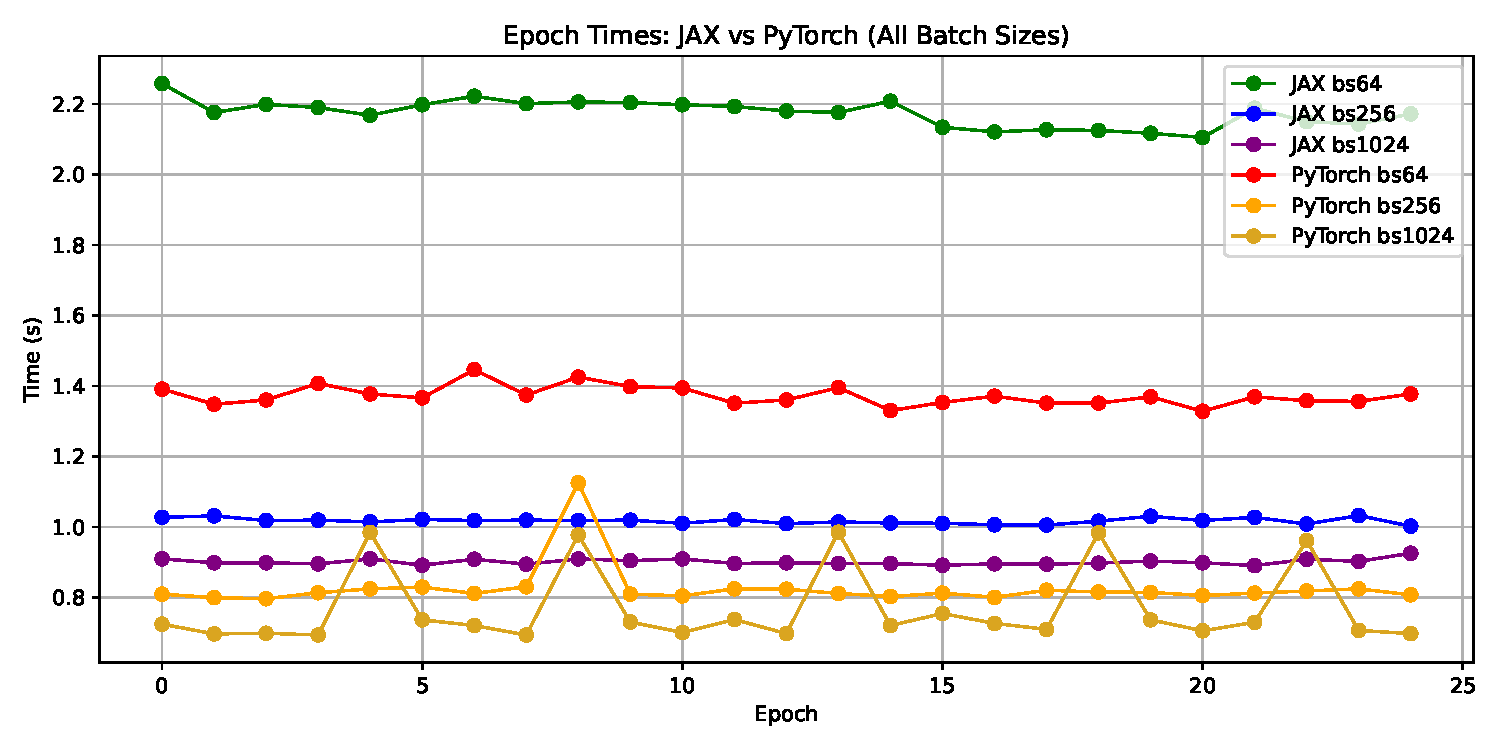
\includegraphics[scale=0.2]{epoch_times_all_curves}
\par\end{centering}

}\subfloat[\label{fig:Training-Time-by-1}Comparison of accuracy (left) and loss
(right). \protect \\
$\ensuremath{\text{ }}$$\ensuremath{\text{ }}$$\ensuremath{\text{ }}$$\ensuremath{\text{ }}$$\ensuremath{\text{ }}$The
left most images are for JAX, and right most images are for Torch. ]{\begin{centering}
\begin{tabular}{c}
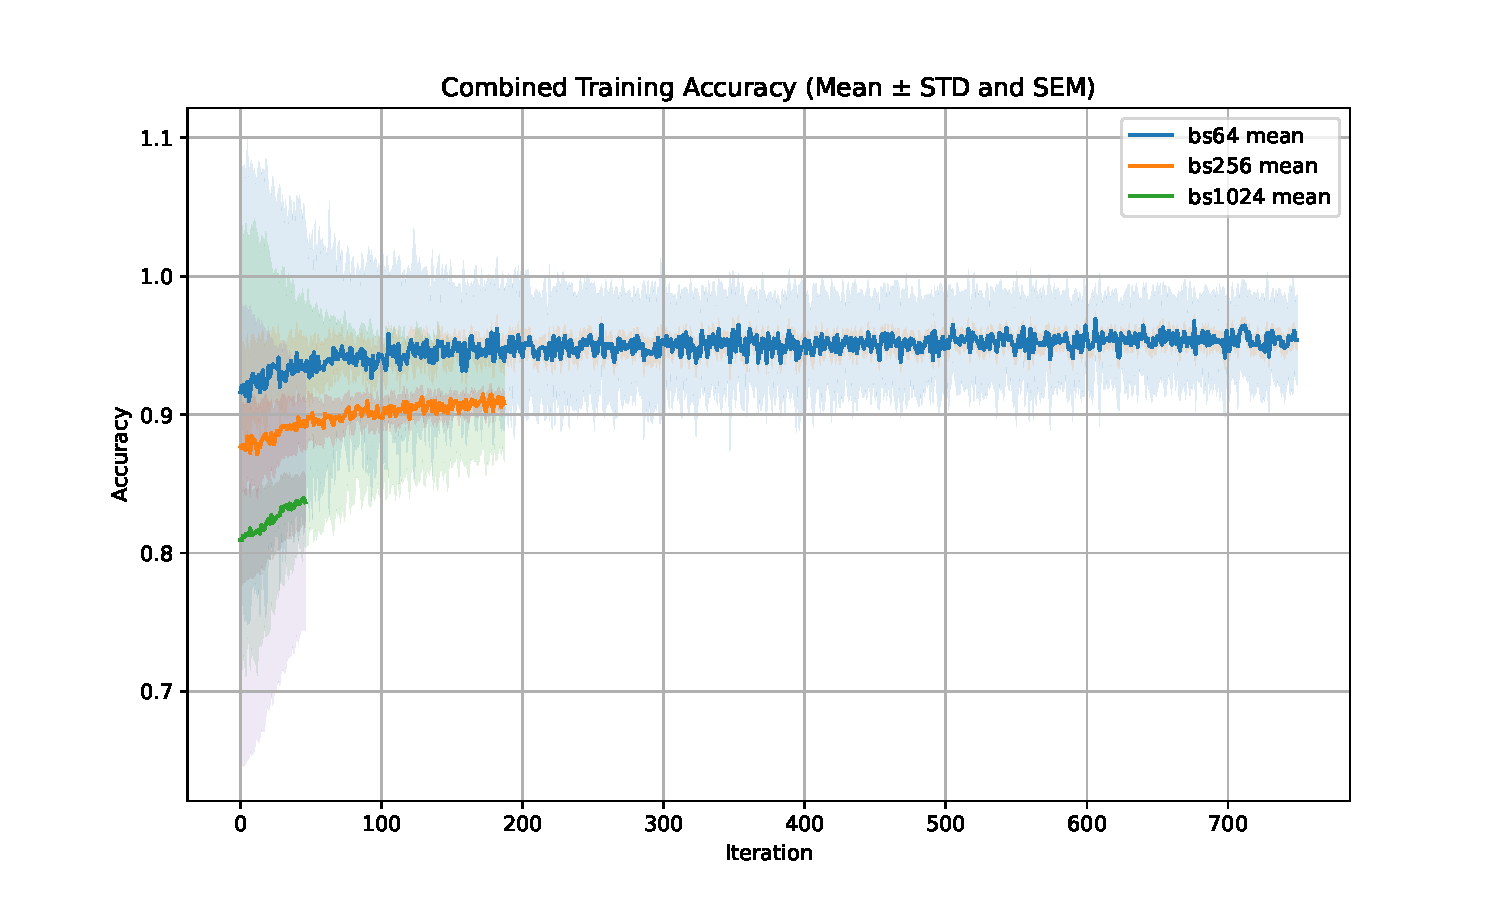
\includegraphics[scale=0.2]{combined_accuracy_with_std_sem}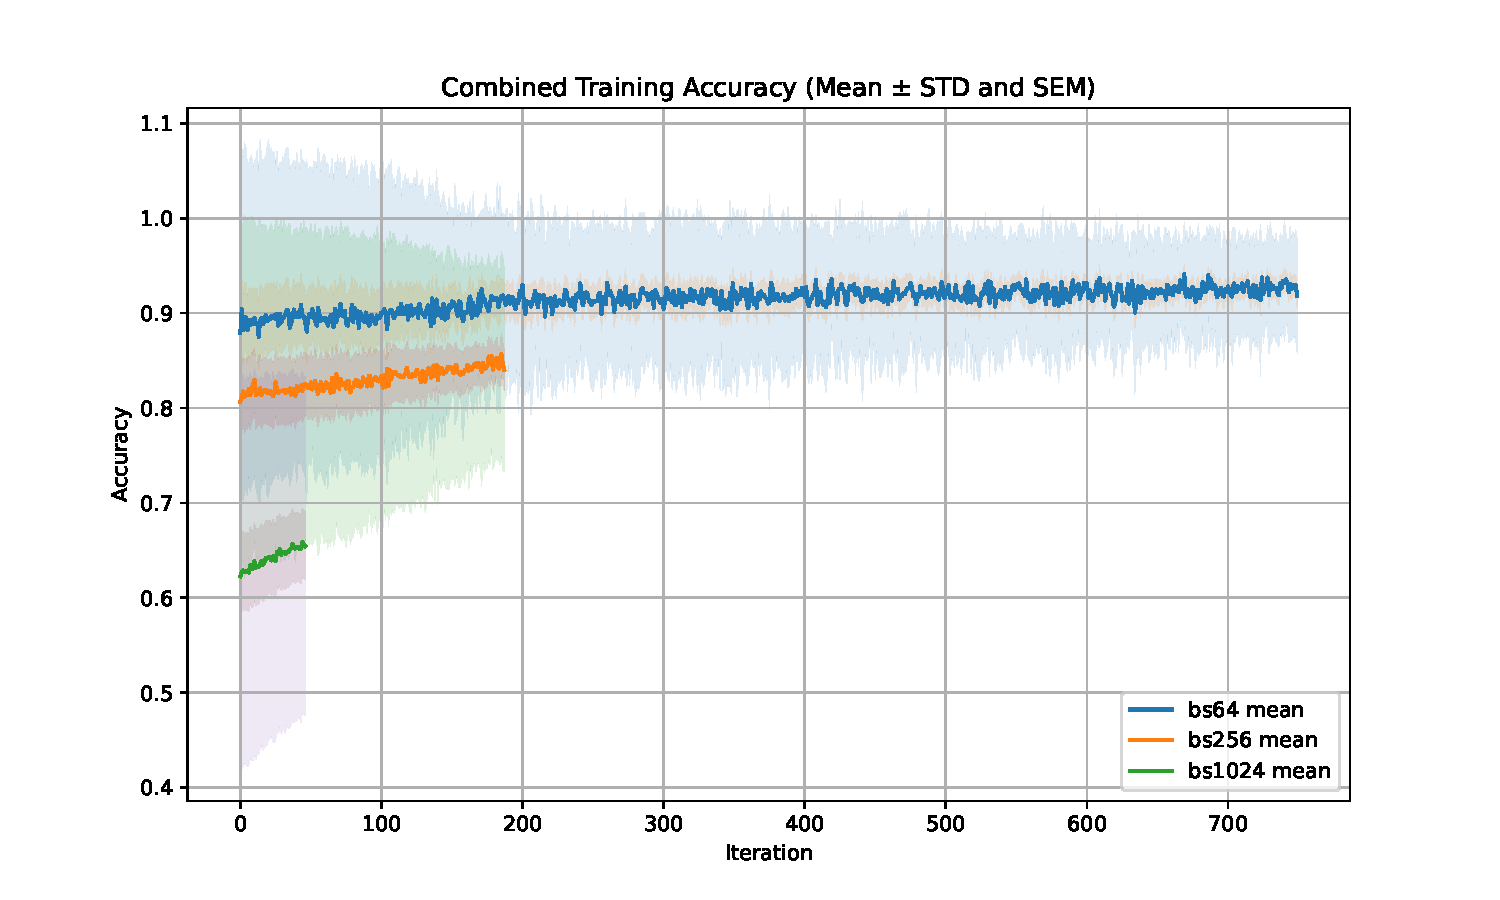
\includegraphics[scale=0.2]{combined_pytorch_accuracy_with_std_sem}\tabularnewline
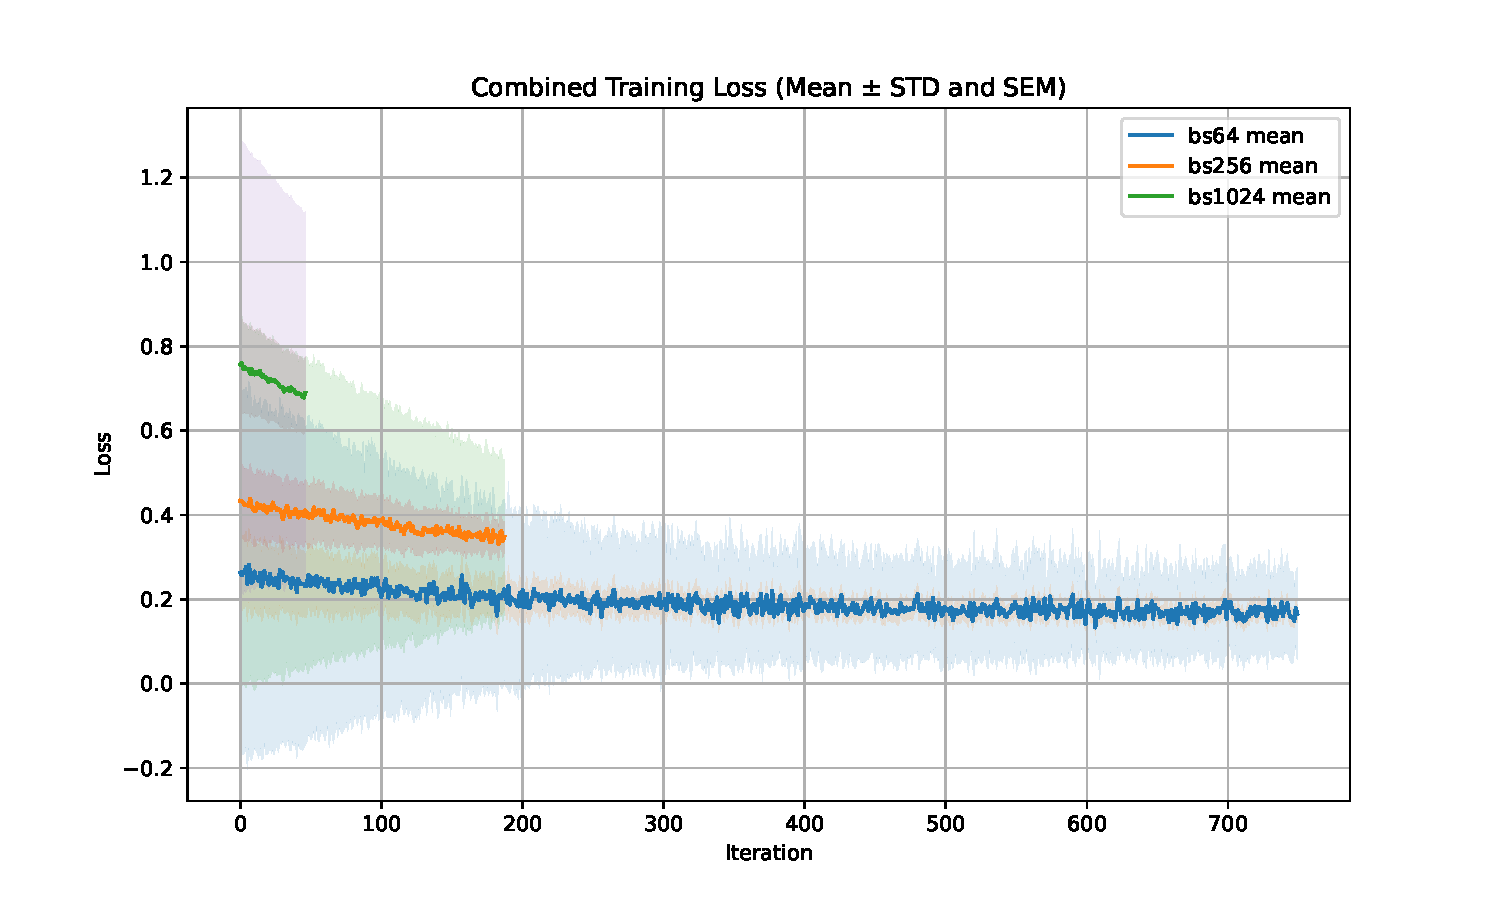
\includegraphics[scale=0.2]{combined_loss_with_std_sem} 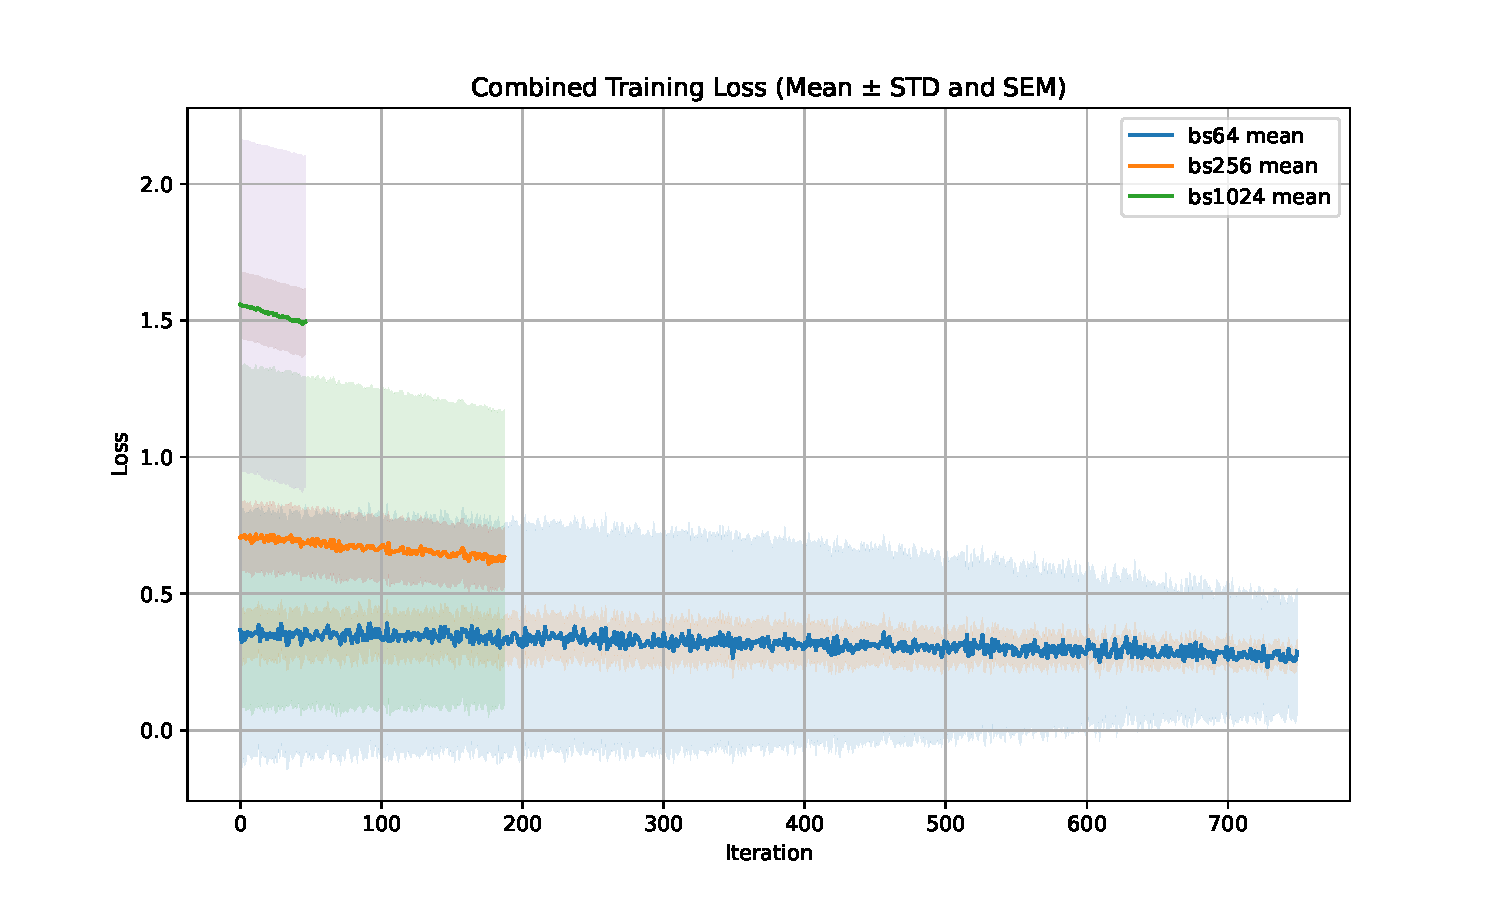
\includegraphics[scale=0.2]{combined_pytorch_loss_with_std_sem}\tabularnewline
\end{tabular}
\par\end{centering}
\begin{centering}
\par\end{centering}
}
\par\end{centering}
\caption{Performance and Accuracy/Loss Comparison}

\end{figure}
\end{sol*}
\begin{question}
Reflect on your experience: What was easier/harder in JAX vs PyTorch/TensorFlow?
\begin{sol*}
In retrospect, both were of similar difficulty, though JAX took much
longer to implement due to my personal lack of experience with the
framework. I do find Pytorch to be a bit more intuitive, but that
might by my own bias towards object oriented frameworks over functional
ones. Research wise, I find it easier to work in Pytorch because there
is a much more robust library of online resources related to the library.
Broadly speaking, training, optimization, and logging metrics is fairly
similar across the two libraries regardless of their different programming
paradigms. 
\end{sol*}
\begin{question}
Compare the performance of the two frameworks.
\end{question}

\begin{sol*}
The performance of the two frameworks was very similar, as can be
seen in figure \ref{fig:Training-Time-by-1}. The initial accuracy
was a bit lower for Jax than Tensorflow, but this might be due to
the slightly different random seeds used between the two frameworks
as they use different processes for setting random seeds. The overall
training results seem broadly similar and comparable between the two
frameworks. JAX seems to have performed significantly better with
a larger batch size in terms of accuracy and loss, which suggests
that its superior XLA compilation model may benefit model training.
However, more experimentation would be required before drawing any
broad conclusions.
\end{sol*}
\end{question}

\end{question}


\section{AI Disclosure and Note}

The Syllabus states ``Assignments \& Presentations: Use of AI tools
(e.g., ChatGPT, Gemini, Copilot) are not permitted.'' As such, my
response to the questions ``What did AI suggest? What did you accept/reject
and why?'' is that AI use is not permitted for assignments (per the
syllabus), and that therefore it was not used. 

If the policy for the course regarding use of AI in assignments has
changed, I would request that you please make an announcement clarifying
in what ways AI can be used for assignments.

\section{References}

$\ensuremath{\text{ }}$

{[}1{]} A. Kafesu, \textquotedblleft JAX vs. PyTorch: Differences
and Similarities {[}2025{]},\textquotedblright{} Geekflare, Dec. 30,
2024. Accessed: Feb. 13, 2026. {[}Online{]}. Available: https://geekflare.com/dev/jax-vs-pytorch/

{[}2{]} A. Nawaz, \textquotedblleft jit, grad, and vmap in JAX ---
One simple idea behind all three: transforming functions,\textquotedblright{}
Medium, Jan. 26, 2026. Accessed: Feb. 13, 2026. {[}Online{]}. Available:
https://medium.com/@AliPythonDev/jit-grad-and-vmap-in-jax-one-simple-idea-behind-all-three-transforming-functions-ed4734f0eb16

{[}3{]} K. Heckel and J. E. Pedersen, \textquotedblleft Optimizing
GPU/TPU Code With JAX and Pallas,\textquotedblright{} Open Neuromorphic,
Oct. 15, 2024. {[}Online{]}. Available: https://open-neuromorphic.org/neuromorphic-computing/software/hacking-hours/kade-heckel-jax-pallas-optimization/
\end{document}
